\section{Growth diagram bijections}
\label{sec:growth-diagrams}

In this section we recall Sundaram's bijection (using Roby's
description~\cite{MR2716353} based on Fomin's growth
diagrams~\cite{MR1314558}) between oscillating tableaux and
matchings. We also present a new bijection, in the same spirit,
between alternating tableaux and partial permutations. In both
cases, the action of the cactus group on highest weight words becomes
particularly transparent when using Fomin's growth diagrams and local
rules for the Robinson--Schensted correspondence.

\begin{figure}[h]
 \def\arraystretch{1.5}
 \begin{tabular}{rccc}
 &
 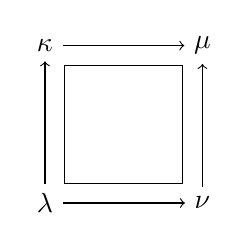
\begin{tikzpicture}[baseline={([yshift=-.5ex]current bounding box.center)},scale=2]
 \node (ka) at (0,1) {$\kappa$};
 \node (la) at (0,0) {$\lambda$};
 \node (nu) at (1,0) {$\nu$};
 \node (mu) at (1,1) {$\mu$};
 \draw[<-] (ka) -- (la);
 \draw[<-] (mu) -- (nu);
 \draw[->] (la) -- (nu);
 \draw[->] (ka) -- (mu);
 \node at (0.5,0.5)[rectangle,minimum size=1.5cm,draw] {};
 \end{tikzpicture}
 &or 
 &
 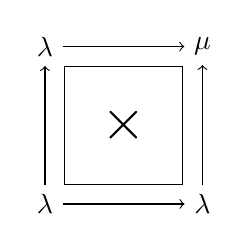
\begin{tikzpicture}[baseline={([yshift=-.5ex]current bounding box.center)},scale=2]
 \node (ka) at (0,1) {$\lambda$};
 \node (la) at (0,0) {$\lambda$};
 \node (nu) at (1,0) {$\lambda$};
 \node (mu) at (1,1) {$\mu$};
 \draw[<-] (ka) -- (la);
 \draw[<-] (mu) -- (nu);
 \draw[->] (la) -- (nu);
 \draw[->] (ka) -- (mu);
 \node at (0.5,0.5)[rectangle,minimum size=1.5cm,draw] {\huge$\times$};
 \end{tikzpicture}\\
 forward rules: %
 & $\mu'=\domS(\kappa'+\nu'-\lambda')$ & %
 & $\mu = \lambda + e_1$\\
 backward rules: %
 & $\lambda'=\domS(\kappa'+\nu'-\mu')$ & %
 & $\lambda = \mu - e_1$ %
 \end{tabular}
 \caption{Cells of a growth diagram and corresponding local rules.}
 \label{fig:growth-cell}
\end{figure}

For our purposes, a growth diagram is a finite collection of cells,
arranged in the form of a Ferrers diagram using the French
convention, as for example in Figures~4
and ~5. Let us first describe the
classical setup, which we use to describe Sundaram's correspondence.

In this case, each cell is either empty or contains a cross.
Moreover, we require that in every row and every column of the growth
diagram there is at most one cell which contains a cross. Every
corner of a cell is labelled with a partition such that the local
rules in Figure~\ref{fig:growth-cell} are satisfied, where
$\lambda^\prime$ denotes the partition conjugate to~$\lambda$
and~$e_1$ is the first unit vector. Moreover, we require that two
adjacent partitions (as for example~$\lambda$ and~$\kappa$ in
Figure~\ref{fig:growth-cell}) either coincide or the one at the head
of the arrow is obtained from the other by adding a unit vector.

Furthermore, we require that the partitions labelling the corners of
a cell satisfy the forward and backward rules of
Figure~\ref{fig:growth-cell}. In fact, the two \Dfn{forward rules}
determine~$\mu$ given the other three partitions and the content of
the cell. The two \Dfn{backward rules} determine the content of the
cell and the partition~$\lambda$ in the bottom-left given the other
three partition.

Thus, the information in a growth diagram is redundant. In
particular, given the partitions labelling the corners along the
bottom-left border and the contents of the cells, one can recover the
remaining partitions. Conversely, given the partitions labelling the
corners along the top-right border of a diagram, one can recover the
remaining partitions and the contents of the cells.

The presentation of the local rules in Figure~\ref{fig:growth-cell}
is slightly non-standard. It has the benefit that the local rule for
empty cells is very similar to the special case of
Definition~\ref{def:local-rules} corresponding to Cartan type~$A_n$,
with two important differences. The first difference is that all
partitions are transposed, the second, that the orientation of the
vertical arrows is reversed.

